\documentclass[12pt]{article}
% \usepackage[top=1in,left=1in, right = 1in, footskip=1in]{geometry}
\usepackage[top=1in,footskip=1in]{geometry}

\usepackage{graphicx}
\usepackage{xspace}
%\usepackage{adjustbox}

\usepackage{pdflscape}

\usepackage{grffile}

\newcommand{\comment}{\showcomment}
%% \newcommand{\comment}{\nocomment}

\newcommand{\showcomment}[3]{\textcolor{#1}{\textbf{[#2: }\textsl{#3}\textbf{]}}}
\newcommand{\nocomment}[3]{}

\newcommand{\swp}[1]{\comment{magenta}{SWP}{#1}}

\newcommand{\eref}[1]{Eq.~(\ref{eq:#1})}
\newcommand{\fref}[1]{Fig.~\ref{fig:#1}}
\newcommand{\Fref}[1]{Fig.~\ref{fig:#1}}
\newcommand{\sref}[1]{Sec.~\ref{#1}}
\newcommand{\frange}[2]{Fig.~\ref{fig:#1}--\ref{fig:#2}}
\newcommand{\tref}[1]{Table~\ref{tab:#1}}
\newcommand{\tlab}[1]{\label{tab:#1}}
\newcommand{\seminar}{SE\mbox{$^m$}I\mbox{$^n$}R}

\usepackage{amsthm}
\usepackage{amsmath}
\usepackage{amssymb}
\usepackage{amsfonts}
\usepackage[utf8]{inputenc} % make sure fancy dashes etc. don't get dropped

\usepackage{lineno}
\linenumbers

\usepackage[pdfencoding=auto, psdextra]{hyperref}

\usepackage{natbib}
\bibliographystyle{unsrt}
\date{\today}

\usepackage{xspace}
\newcommand*{\ie}{i.e.\@\xspace}

\usepackage{color}

\newcommand{\Rx}[1]{\ensuremath{{\mathcal R}_{#1}}\xspace} 
\newcommand{\RR}{\ensuremath{{\mathcal R}}\xspace}
\newcommand{\Rres}{\Rx{\mathrm{res}}}
\newcommand{\Rinv}{\Rx{\mathrm{inv}}}
\newcommand{\Rhat}{\ensuremath{{\hat\RR}}}
\newcommand{\Rt}{\ensuremath{{\mathcal R}(t)}\xspace}
\newcommand{\tsub}[2]{#1_{{\textrm{\tiny #2}}}}
\newcommand{\dd}[1]{\ensuremath{\, \mathrm{d}#1}}
\newcommand{\dtau}{\dd{\tau}}
\newcommand{\dx}{\dd{x}}
\newcommand{\dsigma}{\dd{\sigma}}

\newcommand{\rx}[1]{\ensuremath{{r}_{#1}}\xspace} 
\newcommand{\rres}{\rx{\mathrm{res}}}
\newcommand{\rinv}{\rx{\mathrm{inv}}}

\newcommand{\psymp}{\ensuremath{p}} %% primary symptom time
\newcommand{\ssymp}{\ensuremath{s}} %% secondary symptom time
\newcommand{\pinf}{\ensuremath{\alpha_1}} %% primary infection time
\newcommand{\sinf}{\ensuremath{\alpha_2}} %% secondary infection time

\newcommand{\psize}{{\mathcal P}} %% primary cohort size
\newcommand{\ssize}{{\mathcal S}} %% secondary cohort size

\newcommand{\gtime}{\tau_{\rm g}} %% generation interval
\newcommand{\gdist}{g} %% generation-interval distribution
\newcommand{\idist}{\ell} %% incubation-period distribution

\newcommand{\total}{{\mathcal T}} %% total number of serial intervals

\usepackage{lettrine}

\newcommand{\dropcapfont}{\fontfamily{lmss}\bfseries\fontsize{26pt}{28pt}\selectfont}
\newcommand{\dropcap}[1]{\lettrine[lines=2,lraise=0.05,findent=0.1em, nindent=0em]{{\dropcapfont{#1}}}{}}

\begin{document}

\begin{flushleft}{
	\Large
	\textbf\newline{
		Susceptible host dynamics explain pathogen resilience
	}
}
\newline
\\
Sang Woo Park, \dots, Sarah Cobey
\\
\bigskip
\end{flushleft}

\section*{Abstract}

Major priority for epidemiological research in the time of anthropogenic change is understanding how infectious disease dynamics respond to perturbations.
Interventions to slow the spread of COVID-19 significantly disrupted the transmission of other human pathogens, providing unique opportunities to learn about pathogen characteristics from spatiotemporal variation in re-emergence patterns. 
As interventions lifted, a key question of whether and when respiratory pathogens would eventually return to their pre-pandemic dynamics remains to be answered. 
To address this gap, we develop a framework for estimating pathogen resilience based on how fast epidemic patterns return to their pre-pandemic, endemic dynamics.
Our analysis reveals a possibility that some pathogens may have settled to endemic cycles that are different from their pre-pandemic patterns.
Finally, we show that the replenishment rate of the susceptible pool is a key determinant of pathogen resilience.
Our framework offers a novel perspective to characterizing the dynamics of endemic pathogens and their responses to COVID-19 interventions.

\pagebreak

Understanding how ecological systems respond to perturbations is a fundamental challenge in predicting species persistence and extinction \citep{bender1984perturbation,ives2007stability,scheffer2009early}.
These responses can be characterized in terms of resilience, which often measures how fast a system returns to its stable, reference state following a perturbation \citep{pimm1979structure, neubert1997alternatives,gunderson2000ecological,dakos2022ecological}.
Both theoretical and empirical efforts to quantify resilience of ecological systems have provided key insights for understanding the dynamics of complex systems and linking these findings to actionable strategies for species conservation \citep{chambers2019operationalizing}.
However, despite rich literature on ecological resilience, there have been limited applications to measuring the resilience of host-pathogen systems, especially for human pathogens.

Non-pharmaceutical interventions (NPIs) to slow the spread of COVID-19 disrupted the transmission of other human pathogens, providing large-scale natural experiments for understanding how various host-pathogen systems respond to perturbations \citep{baker2020impact,gomez2021uncertain,koltai2022determinants,park2024predicting}.
In particular, as interventions lifted, large heterogeneities in outbreak dynamics were observed across different pathogens in different countries (Figure 1), likely reflecting differences in NPI patterns, pathogen characteristics, immigration/importation from other countries, and pre-pandemic pathogen dynamics \citep{chow2023effects}.
Even though more than four years have already passed since the emergence of COVID-19, current circulation patterns for many respiratory pathogens appear to be different from their pre-pandemic, seasonal patterns, especially in Hong Kong and Korea:
some pathogens, such as human metapneumovirus and bocavirus in Korea, are circulating at lower levels, whereas other pathogens, such as RSV in Korea, seem to exhibit different seasonality (Figure 1).
These observations pose two fundamental questions for current and future infectious disease dynamics: (1) can we learn about underlying pathogen characteristics, such as their transmissibility or duration of immunity, from re-emergence patterns? and (2) can we predict whether and when other respiratory pathogens will eventually return to their pre-pandemic dynamics?

\begin{figure}[!th]
\includegraphics[width=\textwidth]{../figure1/figure1.pdf}
\caption{
\textbf{Observed heterogeneity in responses to COVID-19 pandemic across respiratory pathogens and norovirus in (A) Canada, (B) Hong Kong, (C) Korea, and (D) US.}
Red points and lines represent data before 2020.
Blue points and lines represent data since 2020.
Gray lines and shaded regions represent the mean seasonal patterns and corresponding 95\% confidence intervals based on the observed outbreak patterns before 2020.
}
\end{figure} 

To address this question, we propose a framework for characterizing the resilience of a host-pathogen system based on how fast the system recovers from perturbation.
We begin by laying out a few representative scenarios that capture the potential impact of COVID-19 interventions on endemic pathogen dynamics and illustrating how resilience can be measured by comparing the pre- and post-pandemic dynamics of susceptible and infected hosts.
In practice, information on susceptible hosts are often unavailable, and traditional methods for reconstructing the dynamics of susceptible hosts require long-term endemic time series \citep{bobashev2000reconstructing,finkenstadt2000time}, which cannot be applied due to disruptions in epidemic patterns caused by COVID-19 interventions.
Instead, we utilize Takens' embedding theorem to reconstruct empirical attractors from data and further measure the distance from this empirical attractor \citep{takens2006detecting}.
This reconstruction allows us to characterize the rate at which this distance decreases over time, which correspond to pathogen resilience.
We apply this framework to analyzing pathogen surveillance data for a wide array of respiratory and non-respiratory pathogens from Canada, Hong Kong, Korea, and US.
Finally, we show that susceptible host dynamics are a key determinants of pathogen resilience.
Our study offers unique insights into understanding pathogen re-emergence patterns following COVID-19 interventions.
% \swp{Revisit.}
 
\section*{Conceptual introduction to pathogen resilience}

In classical ecological literature, resilience of an ecological system is measured by the rate at which the system returns to its reference state following a perturbation \citep{pimm1979structure, neubert1997alternatives,gunderson2000ecological,dakos2022ecological}.
This rate corresponds to the largest real part of the eigenvalues of the linearized system near equilibrium---here, we refer to this value as the \emph{intrinsic} resilience of the system, which represents the expected rate of return from perturbed states.
However, respiratory pathogens often exhibit seasonal variation in transmission, meaning that the intrinsic resilience of a host-pathogen system varies across season.
Nonetheless, we can still measure the \emph{empirical} resilience of a host-pathogen system by looking at how fast the system returns to the pre-pandemic, endemic dynamics after interventions are lifted.

As an example, consider an intervention that reduce transmission by 50\% for 6 months starting in 2020, which causes epidemic patterns to deviate from its original stable annual cycle for a short period of time and eventually come back (Figure 2A).
To measure the empirical resilience of this system, we first need to be able to measure the distance from its pre-pandemic attractor.
There are many different ways we can measure the distance from attractor, but for illustrative purposes, we choose one of the most parsimonious approach: that is, we look at how the susceptible (S) and infected (I) populations change over time and measure the distance on the SI phase plane (Figure 2B).
In this simple case, the locally estimated scatterplot smoothing (LOESS) fit indicates that the distance from attractor decreases linearly on average (Figure 2C).
Furthermore, the overall rate of return matches the intrinsic resilience of the seasonally unforced system (Figure 2C).

\begin{figure}[!th]
\includegraphics[width=\textwidth]{../figure2/figure2_simple.pdf}
\caption{
\textbf{Conceptual framework for measuring pathogen resilience following NPIs across different scenarios.}
(A, D, G) Simulated epidemic trajectories across various models. 
Red and blue solid lines represent epidemic dynamics before and after interventions are introduced, respectively.
Red dashed lines represent counterfactual epidemic dynamics in the absence of interventions.
Gray regions indicate the duration of interventions.
(B, E, H) Phase plane representation of the corresponding model.
Red and blue solid lines represent epidemic trajectories on an SI phase plane before and after interventions are introduced, respectively.
(C, F, I) Changes in logged distance from attractor over time.
Blue lines represent the logged distance from attractor.
Orange lines represent the locally estimated scatterplot smoothing (LOESS) fits to the logged distance from attractor.
Dotted lines are superimposed as a comparison to have the same slope as the intrinsic resilience of the seasonally unforced system.
}
\end{figure}

Alternatively, NPIs can permanently change our behavior and have persisting impact on the pathogen dynamics; 
as an example, we consider a scenario in which a 10\% reduction in transmission persists even after the NPIs are lifted (Figure 2D--F).
In such cases, we cannot know whether the pathogen will return to its original cycle or a different cycle until many years have passed after the NPIs are lifted, meaning that we cannot measure the distance against the new attractor that the system will eventually approach.
Nonetheless, we can still measure the distance against the original, pre-pandemic attractor and ask how the distance changes over time (Figure 2E).
The LOESS fit suggests that the distance from the attractor will initially decrease exponentially on average (equivalently, linearly on a log scale) and eventually plateau (Figure 2F).
Here, a permanent 10\% reduction in transmission rate slows down the system, which causes the distance from the attractor to decrease at a slower rate (Figure 2F) than it would have otherwise in the absence of permanent transmission reduction (Figure 2C).
This example shows that resilience is not necessarily an intrinsic property of a specific pathogen.
Instead, pathogen resilience is a property of a specific attractor that a host-pathogen system approaches, which depends on both pathogen and host characteristics.
% \swp{Add discussion about observation error, e.g., under-reporting.}

Finally, transient phenomena can also complicate the picture (Figure 2G--I).
For example, a stage-structured model for RSV initially exhibits a stable annual cycle, but perturbations from NPIs cause the epidemic to exhibit biennial cycles (Figure 2G).
Despite this biennial cycle, we see that the system eventually approaches the original pre-pandemic attractor (Figure 2H), suggesting that this biennial cycle is a transient phenomenon.
The LOESS fit indicates that the distance from the attractor will initially decrease exponentially at a rate that is consistent with the intrinsic resilience of the seasonally unforced system, but the rate of decrease slows down as the epidemic exhibits a biennial cycle (Figure 2I).
In classical ecological theory, this behavior is also referred to as a ghost attractor, which causes long transient dynamics and slow transitions \citep{hastings2018transient}.
As we show in Supplementary Figure S1, strong seasonal forcing in transmission can also lead to transient phenomena for a simple SIRS model, causing a slowing down of the system.

In Supplementary Materials, we also explore measuring the resilience of a two-strain host-pathogen system:
when the dynamics two strains (or two pathogens) are coupled through cross immunity, we would expect the entire system to be characterized by a single resilience value (rather than having two separate resilience for each strain).
Simulations from a simple two-strain system illustrate that separate analyses of individual strain dynamics (e.g., RSV A vs B) and a joint analysis of total infections (e.g., total RSV infections) yield identical resilience estimates, confirming our expectation (Supplementary Figure S2, 3).
Analogous to a single system, strong seasonal forcing in transmission can cause the system to slow down through transient phenomena (Supplementary Figure S4).

These observations indicate three possibilities.
First, we can directly estimate the empirical resilience of a host-pathogen system by looking at how fast the system approaches a pre-pandemic attractor, provided that we can measure the distance from attractor.
The empirical approach to estimating pathogen resilience is particularly convenient because it does not require us to know the true underlying model.
As we show in Supplementary Figure S5, estimating the intrinsic resilience from fitting standard compartmental models can lead to biased estimates, especially under model misspecification.
Second, resilience estimates allow us to make phenomenological predictions about the dynamics of a host-pathogen system following a perturbation:
assuming that the distance from the attractor will decrease exponentially over time, we can obtain a ballpark estimate for when the system will reach an attractor.
Finally, deviation from an exponential decrease in the distance from attractor can provide information about whether the system has reached an alternative attractor, or a ghost attractor, that is different from the original, pre-pandemic attractor.
These alternative attractors may reflect continued perturbations from permanent changes in transmission patterns as well as changes in immune landscapes.

\section*{Inferring pathogen resilience from real data}

Based on these observations, we now set out to infer pathogen resilience from real data.
Here, we briefly lay out our approach to estimating pathogen resilience from real data (Figure 3).
We then test this approach against simulations and apply it to real data.

So far, we focused on simple examples that assume a constant transmission reduction.
However, in practice, the impact of NPIs on pathogen transmission is likely more complex (Figure 3A), reflecting introduction and relaxation of various intervention strategies.
These complexities can lead to longer delays between the introduction of NPIs and pathogen re-emergence as well as temporal variation in outbreak sizes (Figure 3B):
in this example, continued transmission reduction from NPIs limits the size of the first outbreak in 2021 following the emergence, allowing for a larger outbreak in 2022 when NPIs are further relaxed.

Previously, we relied on the dynamics of susceptible and infected hosts to compute the distance from attractor (Figure 2), but information on susceptible hosts are often not available in practice.
In addition, uncertainties in case counts due to observation error as well as the possibility of complex, multiannual attractor adds challenges to measuring the distance from attractor.
To address these challenges, we first reconstruct an empirical attractor by utilizing Takens' theorem, which states that an attractor of a nonlinear multidimensional system can be mapped onto a delayed embedding \citep{takens2006detecting}.
Here, we use delayed copies of logged values of pre-pandemic cases $C(t)$ (Figure 3C) to reconstruct the attractor:
\begin{equation}
\langle\log(C(t)+1), \log(C(t-\tau)+1), \dots, \log(C(t-(M-1)\tau)+1)\rangle,
\end{equation}
where the delay $\tau$ and embedding dimension $M$ are determined based on autocorrelations and false nearest neighbors, respectively \citep{kennel1992determining,tan2023selecting}.
We then apply the same delay and embedding dimensions to the entire time series to determine the position on a multi-dimensional state space (Figure 3D), which allows us to measure the nearest neighbor distance between the current state of the system and the empirical attractor (Figure 3E).
In principle, we can quantify how fast this distance decreases by fitting a linear regression on a log scale, where the slope of the linear regression corresponds to pathogen resilience.
As we show in Supplementary Figure S6, overall temporal variations in the distance from attractor, especially the observed rate of decrease, appear robust to choices about embedding delays and dimensions; 
we note that using longer delays and higher dimensions tend to smooth out temporal variations in the distance from attractor.

\begin{figure}[!ht]
\includegraphics[width=\textwidth]{../figure3/figure3.pdf}
\caption{
\textbf{A schematic diagram explaining how pathogen resilience can be inferred from real data.}
(A) A realistic example of a synthetic NPI, represented by a relative reduction in transmission.
(B) The impact of the synthetic NPI on epidemic dynamics simulated using a stochastic SIRS model.
(C) Generating delayed copies of the logged time series allows us to obtain an embedding.
(D) Two dimensional representation of an embedding.
(E) Delayed embedding allows us to calculate the nearest neighbor distance from the empirical attractor, which is determined based on the pre-pandemic time series.
This distance time series can be used to infer pathogen resilience by fitting a linear regression after choosing an appropriate window for regression.
}
\end{figure}

Complex changes in the distance from attractor suggest that estimating pathogen resilience from linear regression will likely be sensitive to our choice of fitting windows for the regression.
In Supplementary Materials, we explore an automated window selection criteria for linear regression and test it against randomized, stochastic simulations across a wide range of realistic NPI shapes.
We find that resilience estimates based on the automated window selection criteria are moderately correlated (0.54) with the intrinsic resilience of the post-NPI attractor (Supplementary Figure S7).
In contrast, a naive approach that uses the entire time series, starting from the peak distance, only gives a correlation of 0.21 and consistently underestimates the intrinsic resilience (Supplementary Figure S7).

% A closer observation of the resulting time series of the distance from attractor provides three important insights (Figure 3E).
% First, the relaxation of NPIs in realistic settings can cause a false return of the system, as indicated by a rapid decrease in the distance in early 2022 followed by a rapid increase in distance.
% In other words, we need at least several years of data to be able to properly assess the return of system to an attractor.
% Second, complex changes in the distance from attractor suggests that estimating pathogen resilience from linear regression will likely be sensitive to our choice of fitting windows for the regression.
% Finally, temporal variation in the impact of NPIs on pathogen transmission will affect the intrinsic resilience of the system throughout the NPI period, meaning that the estimated resilience from linear regression will likely reflect some sort of average impact of the NPIs.

Now, we apply this approach to pathogen surveillance data presented in Figure 1.
For each time series, we apply Takens' theorem independently to reconstruct the empirical attractor and obtain the corresponding time series of distance from attractors (Supplementary Figure S8 for the distance time series and linear regression fits).
Then, we use the automated window selection criteria to fit a linear regression and estimate the empirical resilience for each pathogen in each country.
For most respiratory pathogens, resilience estimates fall between $0.4/\mathrm{year}$ and $1.8/\mathrm{year}$ (Figure 4A), with the exception of Rhinovirus in the US ($0.066/\mathrm{year}$; 95\% CI: $0.018/\mathrm{year}$--$0.113/\mathrm{year}$) and Bocavirus in Korea ($0.087/\mathrm{year}$; 95\% CI: $0.023/\mathrm{year}$--$0.151/\mathrm{year}$).
Excluding these exceptions, the mean resilience of common respiratory pathogens is $0.974/\mathrm{year}$ (95\% CI: $0.784/\mathrm{year}$--$1.16/\mathrm{year}$).
As a reference, this is $\approx 7$ times higher than the intrinsic resilience of pre-vaccination measles dynamics ($\approx 0.13/\mathrm{year}$).
Finally, resilience estimates for norovirus appears to be comparable to the intrinsic resilience of measles: $0.119/\mathrm{year}$ (95\%CI: $0.004/\mathrm{year}$--$0.233/\mathrm{year}$) for Korea and $0.385/\mathrm{year}$ (95\% CI: $0.167/\mathrm{year}$--$0.603/\mathrm{year}$).
A simple ANOVA shows that there are significant differences in resilience estimates across countries ($p<0.036$) and pathogens ($p<0.030$).

\begin{figure}[!th]
\begin{center}
\includegraphics[width=0.8\textwidth]{../figure4/figure4.pdf}
\caption{
\textbf{Summary of resilience estimates.}
(A) Estimated pathogen resilience.
The gray horizontal line represents the intrinsic resilience of pre-vaccination measles dynamics.
(B) Predicted timing of when each pathogen will return to their pre-pandemic cycles.
The dashed line in panel B indicates the end of 2024 (current observation time).
Error bars represent 95\% confidence intervals.
}
\end{center}
\end{figure}

Using resilience estimates, we now predict when each pathogen will return to their original pre-pandemic cycles.
Specifically, we extend our linear regression fits to distance-from-attractor time series and ask when the predicted regression line will cross a threshold value, which we set to a mean of pre-pandemic distances.
We predict that a return to pre-pandemic cycles would be imminent for most pathogens (Figure 4B; see Supplementary Figure S9 for a zoomed out version).
In addition, we also predict that many pathogens should have already returned to their pre-pandemic dynamics by the end of 2024; 
but these predictions contradict some of the observed pathogen dynamics.
For example, we predict that both human metapneumovirus and RSV in Korea should have returned to their attractors by now, but the magnitude and timing of recent epidemics are different from pre-pandemic patterns (Figure 1). 
These observations suggest the possibility that some common respiratory pathogens may have converged to different attractors.

In Supplementary Materials, we also consider using a lower threshold for the false nearest neighbor approach when determining the embedding dimension;
this gives a higher embedding dimension.
As explained earlier (Supplementary Figure S6), this gives a smoother distance-from-attractor time series (compare Supplementary Figure S10 with S8);
this also requires us to use longer time series, which prevents us from estimating resilience for some pathogens.
Overall, resulting estimates of pathogen resilience with higher embedding dimensions still fall between $0.3/\mathrm{year}$ and $2.1/\mathrm{year}$ for the most part (Supplementary Figure S11).
A direct comparison between two approaches (i.e., original estimate vs using higher dimensions) shows a strong consistency in resilience estimates (Supplementary Figure S12).

\section*{Susceptible host dynamics explain variation in pathogen resilience}

So far, we focused on quantifying pathogen resilience from the observed patterns of pathogen re-emergence following COVID-19 interventions.
But what factors determine how resilient a host-pathogen system is?
Here, we use a standard Susceptible-Infected-Recovered-Susceptible (SIRS) model to show that susceptible host dynamics are the key determinants of pathogen resilience.
To do so, we vary the basic reproduction number $\mathcal R_0$, which represents the average number of secondary infections caused by a newly infected individual in a fully susceptible population, and the duration of immunity and compute intrinsic resilience for each parameter.

\begin{figure}[!th]
\begin{center}
\includegraphics[width=\textwidth]{../figure_summary/figure_summary.pdf}
\caption{
\textbf{Linking pathogen resilience to epidemiological parameters and susceptible host dynamics.}
(A) The heat map represents intrinsic resilience as a function of the basic reproduction number $\mathcal R_0$ and the duration of immunity.
(B) The heat map represents per-capita susceptible replenishment rate as a function of the basic reproduction number $\mathcal R_0$ and the duration of immunity.
The standard SIRS model is used to compute intrinsic resilience and per-capita susceptible replenishment rate.
Lines correspond to a set of parameters that are consistent with mean resilience estimates for each pathogen.
Pathogens are ranked based on their mean resilience estimates, averaged across different countries.
}
\end{center}
\end{figure}

We find an increase in $\mathcal R_0$ and a decrease in duration of immunity correspond to an increase in pathogen resilience (Figure 5A).
These variations can be understood in terms of the susceptible host dynamics, where faster per-capita susceptible replenishment rate causes the system to be more resilient (Figure 5B).
This rate can be expressed as a ratio between absolute rate at which new susceptibles enter the population and the equilibrium number of susceptible individuals in the population, $\bar{S}$.
Therefore, both higher $\mathcal R_0$ and shorter duration of immunity can drive faster per-capita susceptible replenishment rate (Figure 5B), especially because higher $\mathcal R_0$ leads to lower $\bar{S}$.

Finally, we can now rank different pathogens based on the average values of empirical resilience, which allows us to determine a set of parameters that are consistent with the estimated resilience (Figure 5A).
Across all pathogens we consider, except for bocavirus and norovirus, we estimate that the average duration of immunity is likely to be short ($<6$ years) across a plausible range of $\mathcal R_0$.
These rankings further allow us to map each pathogen onto a set of parameters that are consistent with its empirical resilience (Figure 5A) and obtain a plausible range of susceptible replenishment rates for each pathogen (Figure 5B).
However, we note that there is no one-to-one correspondence between susceptible replenishment rates and pathogen resilience, leading to a wide uncertainty in the estimates for susceptible replenishment rates (Figure 5B).

\section*{Discussion}

The COVID-19 interventions have caused major disruptions to circulation patterns of both respiratory and non-respiratory pathogens, adding challenges to predicting their future dynamics \citep{baker2020impact,gomez2021uncertain,koltai2022determinants,park2024predicting}.
On the other hand, these interventions offer large-scale natural experiments for understanding how different pathogens respond to perturbations.
In this study, we show that pathogen re-emergence patterns following COVID-19 interventions can be characterized through the lens of ecological resilience.
Traditionally, ecological resilience measures how fast a system returns to a reference state following a perturbation.
In the context of respiratory pathogens, resilience measures how fast epidemics return to their endemic cycles after interventions are lifted.
% Our study demonstrates that this perspective provides unique insights into underlying susceptible host dynamics and allows predictions for when epidemics will return to their endemic cycles.

We use an attractor reconstruction approach to quantify how distance from attractor changes over time for each pathogen \citep{takens2006detecting}.
We show that the resilience of a host-pathogen system can be estimated by fitting a linear regression to a logged distance-from-attractor time series.
Overall, we estimate that the resilience for most common respiratory pathogens ranges between $0.4/\mathrm{year}$ and $1.8/\mathrm{year}$, which is 3--14 times more resilient than prevaccination measles, indicating potential challenges in controlling common respiratory pathogens.

Our framework allows us to make phenomenological predictions about when each pathogen will return to their endemic cycles.
The ability to predict future epidemic patterns from resilience estimates offers a new paradigm for epidemic forecasting.
While this approach cannot predict the exact timing of outbreaks or epidemic patterns, it is nonetheless useful for predicting when epidemics will settle down to regular cycles after a large perturbation, such as COVID-19 interventions.

Our analyses suggest a possibility that several pathogens may have converged to different endemic cycles compared to their pre-pandemic epidemic patterns.
Key examples include human metapnuemovirus, RSV, and bocavirus in Korea as well as RSV in Hong Kong.
These changes may reflect changes in surveillance or actual shift in the dynamics, caused by permanent changes in behavior or population-level immunity.
While it seems unlikely that permanent changes in behavior would only affect a few pathogens and not others, we cannot rule out this possibility given heterogeneity in the age of infection across different respiratory pathogens \swp{CITE}.
A shift in population-level immunity is plausible, as the emergence of SARS-CoV-2 and extinction of influenza B/Yamagata likely caused major changes in immune landscapes;
interactions among co-circulating pathogens, such as cross immunity between RSV and HMPV \citep{bhattacharyya2015cross}, may have also contributed to changes in population-level immunity.
However, we currently do not know how immunity, or lack thereof, from these pathogens would affect infection from other pathogens.
Future studies should use detailed mechanistic models, coupled with behavioral and immunological data, to test these hypotheses and better understand post-pandemic dynamics of endemic pathogens.

We show that susceptible host dynamics shape pathogen resilience, where faster replenishment of the susceptible population causes the pathogen to be more resilient.
For simplicity, we focus on waning immunity and birth as a main driver of the susceptible host dynamics but other mechanisms can also contribute to the replenishment of the susceptible population.
In particular, pathogen evolution, especially the emergence of antigenically novel strains, can cause effective waning of immunity in the population;
therefore, we hypothesize that faster rates of antigenic evolution can also cause a pathogen to be more resilient.
Future studies should explore the relationship between the rate of evolution and resilience for antigenically evolving pathogens.

Quantifying pathogen resilience also offers novel approaches to validating population-level epidemiological models.
So far, the majority of model validation in epidemiology is based on the ability of a model to reproduce the observed epidemic dynamics and to predict future dynamics \citep{grenfell2002dynamics,bhattacharyya2015cross,pitzer2015environmental,dean2018human,pons2018serotype}.
However, there can be plethora of models that meet these criteria.
For example, two major RSV models have been proposed so far to explain biennial epidemic patterns: (1) a stage- and age-structured model that allows for disease severity to vary with number of past infections and age of infection \citep{pitzer2015environmental} and (2) a pathogen-interaction model that accounts for cross immunity between RSV and human metapnuemovirus \citep{bhattacharyya2015cross}.
Since both models can accurately reproduce the observed epidemic patterns, standard criteria for model validation do not allow us to distinguish between these two models from population-level data alone.
Instead, we can measure the empirical resilience of each model by simulating various perturbations and compare them to estimates of empirical resilience from data, using COVID-19 interventions as an opportunity.
Future studies should further investigate using pathogen resilience for validating epidemic models.

There are several limitations to our work.
First of all, we did not extensively explore other approaches to reconstructing the attractor.
Recent studies showed that more sophisticated approaches, such as using non-uniform embedding, can provide more robust reconstruction for noisy data \citep{tan2023selecting}.
In the context of causal inference, choices about embedding can have major impact on the resulting inference \citep{cobey2016limits}.
Our resilience estimates are likely overly confident given a lack of uncertainties in attractor reconstruction as well as the simplicity of our statistical framework.
Short pre-pandemic time series also contributes to the crudeness of our estimates.
Nonetheless, as illustrated in our sensitivity analyses (Supplementary Figure S6, S10--S12), inferences about pathogen resilience appear to be robust to decisions about embedding lags and dimensions---this is because tracking the rate at which the system approaches the attractor is likely a much simpler problem than making inferences about causal directionality.
Our qualitative prediction that common respiratory pathogens are more resilient than prevaccination measles is also likely to be robust to these predictions, given how rapid many respiratory pathogens returned to their original cycles following COVID-19 interventions.
% Despite these limitations, our study illustrates the utility of quantifying pathogen resilience for understanding how different pathogens respond to perturbations.

Predicting the impact of anthropogenic changes on infectious disease dynamics is a fundamental aim of infectious disease research in a rapidly changing world.
Our study illustrates that quantifying pathogen resilience can help us understand how infectious disease pathogens respond to major perturbations caused by public health interventions.
More broadly, a detailed understanding of the determinants of pathogen resilience may offer unique insights into pathogen persistence and controllability.

\section*{Materials and Methods}

\subsection*{Data}

We gathered time series on respiratory infections from four different countries: Canada, Hong Kong, Korea, and United States (US).
As a reference, we also included time series data on norovirus infections for available countries---in contrast to respiratory pathogens, we expect gastrointestinal viruses, such as norovirus, to be less affected by COVID-19 intervention measures.
For all time series, we rounded every year to 52 weeks by taking the average number of cases and tests between the 52nd and 53rd week.
We also rescale all time series to account for changes in testing patterns, which are then used for the actual analysis.

Weekly time series of respiratory infection cases in Canada comes from the Respiratory Virus Detection Surveillance System, which collect data from select laboratories across Canada.
We extract the data from \url{https://www.canada.ca/en/public-health/services/surveillance/respiratory-virus-detections-canada.html}.
To account for an increase in testing from 2013 to 2024, we calculate a 2 year moving average for the number of tests for each pathogen, which we use as a proxy for testing effort.
Then, we divide the smoothed testing patterns by the smoothed value at the final week such that the testing effort has a maximum of 1.
We then divide weekly cases by the testing effort to obtain a scaled case time series.
A similar approach was used earlier for the analysis of RSV time series in the US \citep{pitzer2015environmental}.

Weekly time series of respiratory infection cases in Hong Kong comes from the Centre for Health Protection, Department of Health. 
We extract the data from \url{https://www.chp.gov.hk/en/statistics/data/10/641/642/2274.html}.
We also apply the same scaling procedure to the time series as we did for Canada.
For Hong Kong, we only adjust for testing efforts up to the end of 2019 because there was a major reduction in testing for common respiratory pathogens since 2020.

Weekly time series of acute respiratory infection cases in Korea comes from Korea Disease Control and Prevention Agency.
We extract the data from \url{https://dportal.kdca.go.kr/pot/is/st/ari.do}.
While we do not have information on testing, the reported number of respiratory infections consistently increased from 2013 to the end of 2019, which we interpreted as changes in testing patterns.
Since we do not have testing numbers, we used the weekly sum of all acute respiratory viral infection cases as a proxy for testing, which were further smoothed with moving averaged and scaled to have a maximum of 1.
For Korea, we also only adjust for testing efforts up to the end of 2019.

Finally, weekly time series of respiratory infection cases in the US comes from the National Respiratory and Enteric Virus Surveillance System.
In the US, there has been a large increase in testing against some respiratory pathogens, especially RSV, which could not be corrected for through simple scaling.
Instead, we derive an incidence proxy by multiplying the test positivity with influenza-like illness positivity, which is taken from \url{https://gis.cdc.gov/grasp/fluview/fluportaldashboard.html}.
This method of estimatnig an incidence proxy has been recently applied in the analysis of seasonal coronaviruses \citep{kissler2020projecting} and Mycoplasma pneumoniae infections \citep{park2024predicting}.
Detailed assumptions and justifications are provided in \citep{goldstein2011predicting}.

\subsection*{Estimating pathogen resilience}

In order to measure pathogen resilience from surveillance data, we first reconstruct the empirical pre-pandeic attractor of the system using Takens' embedding theorem \citep{takens2006detecting}.
Specifically, for a given pathogen, we take the pre-pandemic (before 2020) case time series $C(t)$ and reconstruct the attractor using delayed embedding with a uniform delay of $\tau$ and dimension $M$:
\begin{equation}
X_{\tau,m}(t) = \langle\log(C(t)+1), \log(C(t-\tau)+1), \dots, \log(C(t-(M-1)\tau)+1)\rangle.
\end{equation}
Here, the delay $\tau$ is determined by looking at the autocorrelation of the logged pre-pandemic time series and asking when the autocorrelation crosses 0 for the first time \citep{tan2023selecting};
a typical delay for for an annual outbreak is around 13 weeks.

Then, for a given delay $\tau$, we determine the embedding dimension $M$ using the false nearest neighbors approach \citep{kennel1992determining,tan2023selecting}.
To do so, we start with an embedding dimension $e$ and construct a set of points $A_{\tau,e}= \{X_{\tau,e}(t) | t < 2020\}$.
Then, for each point $X_{\tau,e}(t)$, we determine the nearest neighbor from the set $A_{\tau,e}$, which we denote $X_{\tau,e}(\tsub{t}{nn})$ for $t \neq \tsub{t}{nn}$.
Then, if the distance between these two points on $e+1$ dimension, $D_{\tau,e+1}(t) = ||X_{\tau,e+1}(\tsub{t}{nn})-X_{\tau,e+1}(t)||_2$, is larger than their distance on $e$ dimension, $D_{\tau,e}(t) = ||X_{\tau,e}(\tsub{t}{nn})-X_{\tau,e}(t)||_2$, these two points are deemed to be false nearest neighbors;
specifically, we use a threshold $R$ for the ratio between two distances $D_{\tau,e+1}(t)/D_{\tau,e}(t)$ to determine false nearest neighbors.
In the main text, we determine embedding dimension based as the first dimension without any false nearest neighbors for $R=10$.
In Supplementary Matereials, we impose $R=5$ to select for higher dimensions.
Once we determine the embedding lag $\tau$ and dimension $M$, we apply the embedding to the entire time series and calculate the nearest neighbor distance against the attractor $A_{\tau,M}$ to obtain a time series of distance from attractor $D_{\tau,M}(t)$.

From a time series of distance from attractor, we estimate pathogen resilience by fitting a linear regression to an appropriate window.
To automatically select the fitting window, we begin by smoothing the distance time series using locally estimated scatterplot smoothing (LOESS) to obtain $\hat{D}_{\tau,M}(t)$, where the smoothing is performed on a log scale and exponentiated afterwards.
Then, we determine threshold values ($\tsub{T}{start}$ and $\tsub{T}{end}$) for the smoothed distances and choose the fitting window based on when $\hat{D}_{\tau,M}(t)$ crosses these threshold values for the first time.
These thresholds are determined by first calculating maximum distance,
\begin{equation}
\max \hat{D} = \max \hat{D}_{\tau,M}(t),
\end{equation}
and mean pre-pandemic distance,
\begin{equation}
\tsub{\hat{D}}{mean} = \frac{1}{N_{t<2020}} \sum_{t < 2020} \hat{D}_{\tau,M}(t),
\end{equation}
as a reference, and then dividing their ratios into 10 equal bins:
\begin{align}
\tsub{T}{start} &= \tsub{\hat{D}}{mean} \times \left(\frac{\max \hat{D}}{\tsub{\hat{D}}{mean}} \right)^{9/10}\\
\tsub{T}{end} &= \tsub{\hat{D}}{mean} \times \left(\frac{\max \hat{D}}{\tsub{\hat{D}}{mean}} \right)^{1/10}
\end{align}
This allows us to discard the initial period during which the distance increases (from the introduction of intervention measures) and the final period during which the distance plateaus (as the system reaches an attractor).
The fitting window is determined based on when the smoothed distance $\hat{D}_{\tau,M}(t)$ crosses these threshold values for the first time; then, we fit a linear regression to logged (unsmoothed) distances $\log D_{\tau,M}(t)$ using that window.

\subsection*{Mathematical modeling}

Throughout the paper, we use a series of mathematical models to illustrate the concept of pathogen resilience and to understand the determinants of pathogen resilience.
In general, the intrinsic resilience for a given system is given by the largest real part of the eigenvalues of the linearized system at endemic equilibrium.
Here, we focus on the SIRS model and present the details of other models in Supplementary Materials.
The SIRS (Susceptible-Infected-Recovered-Susceptible) model is the simplest model that allows for waning of immunity, where recovered (immune) individuals are assumed to become fully susceptible after an average of $1/\delta$ time period.
The dynamics of the SIRS model is described by the following set of differential equations:
\begin{align}
\frac{\dd S}{\dd t} &= \mu - \beta(t) SI - \mu S + \delta R \\
\frac{\dd I}{\dd t} &= \beta(t) SI - (\gamma + \mu) I \\
\frac{\dd R}{\dd t} &= \gamma I - (\delta + \mu) R \\
\end{align}
where $\mu$ represents the birth/death rate, $\beta(t)$ represents the time-varying transmission rate, and $\gamma$ represents the recovery rate.
The basic reproduction number $\mathcal R_0 = \beta(t)/(\gamma + \mu)$ is defined as the average number of secondary infections caused by a single infected individual in a fully susceptible population and measures the intrinsic transmissibility of a pathogen.

When we first introduce the idea of pathogen resilience (Figure 2), we impose sinusoidal changes to the transmission rate to account for seasonal transmission:
\begin{equation}
\beta(t) = b_1 (1 + \theta \cos(2 \pi (t-\phi))) \alpha(t),
\end{equation}
where $b_1$ represents the baseline transmission rate, $\theta$ represents the seasonal amplitude, and $\phi$ represents the seasonal offset term.
Here, we also introduce an extra multiplicative term $\alpha(t)$ to account for the impact of COVID-19 interventions, where $\alpha(t) < 1$ indicates transmission reduction.
Figure 2A and 2B are generated assuming $b_1 = 3 \times (365/7+1/50)/\mathrm{years}$, $\theta=0.2$, $\phi=0$, $\mu=1/50/\mathrm{years}$, $\gamma=365/7/\mathrm{years}$, and $\delta=1/2/\mathrm{years}$,
In Figure 2A, we impose a 50\% transmission reduction for 6 months from 2020:
\begin{equation}
\alpha(t) = \begin{cases}
0.5 & 2020 \leq t< 2020.5\\
1 & \textrm{otherwise}
\end{cases}
\end{equation}
In Figure 2B, we impose a 50\% transmission reduction for 6 months from 2020 and a permanent 10\% reduction onward:
\begin{equation}
\alpha(t) = \begin{cases}
1 & t < 2020\\
0.5 & 2020 \leq t < 2020.5\\
0.9 & 2020.5 \leq t
\end{cases}
\end{equation}
In both scenarios, we simulate the SIRS model from the following initial conditions ($S(0) = 1/\mathcal R_0$, $I(0) = 1\times 10^{-6}$, and $R(0) = 1 - S(0) - I(0)$) from 1900 until 2030.

To measure the empirical resilience of the SIR model (Figure 2C and 2F), we compute the normalized distance between post-intervention susceptible and logged infected proportions and their corresponding pre-intervention values at the same time of year:
\begin{equation}
\sqrt{\left(\frac{S(t) - \tsub{S}{pre}(t)}{\sigma_S}\right)^2 + \left(\frac{\log I(t) - \log \tsub{I}{pre}(t)}{\sigma_{\log I}}\right)^2},
\end{equation}
where $\sigma_S$ and $\sigma_{\log I}$ represent the standard deviation in the pre-intervention susceptible and logged infected proportions.
We normalize the differences in susceptible and logged infected proportions to allow both quantities to equally contribute to the changes in distance from attractor.
In Supplementary Materials, we also compare the how the degree of seasonal transmission affects empirical resilience by varying $\theta$ from 0 to 0.4; when we assume no seasonality ($\theta = 0$), we do not normalize the distance because the standard deviation of pre-intervention dynamics are zero. 

Finally, we use the SIRS model to understand how underlying epidemiological parameters affect pathogen resilience and link this relationship to underlying susceptible host dynamics.
For the simple SIRS model without seasonal transmission ($\theta = 0$), the intrinsic resilience corresponds to:
\begin{equation}
-\frac{\mathrm{Re}(\lambda)}{2} = \frac{\delta + \beta I^{\ast} + \mu}{2}.
\end{equation}
Here, $I^{\ast}$ represents the prevalence values at endemic equilibrium:
\begin{equation}
I^{\ast} = \frac{(\delta + \mu)(\beta - (\gamma + \mu))}{\beta(\delta + \gamma + \mu)}.
\end{equation}
The susceptible replenishment rate is given by:
\begin{equation}
\tsub{S}{replenish} = \frac{\mu + \delta R}{S^\ast},
\end{equation}
where $S^\ast = 1/\mathcal R_0$ represents the equilibrium proportion of susceptible individuals.
We vary the basic reproduction number $\mathcal R_0$ between 1.1 to 6 and the average duration of immunity $1/\delta$ between 2 to 80 years, and compute these two quantities.
In doing so, we fix all other parameters: $\mu=1/80/\mathrm{years}$ and $\gamma=365/7/\mathrm{years}$.

\pagebreak


\setcounter{figure}{0}
\setcounter{equation}{0}
\renewcommand{\thefigure}{S\arabic{figure}}
\renewcommand{\theequation}{S\arabic{equation}}

\section*{Supplementary Text}

\subsection*{Resilience of a stage-structured system.}

In Figure 2G--I, we use a more realistic, stage-structured model to illustrate how transient phenomena can cause the system to slow down.
Specifically, we use the stage-structured RSV model proposed by \citep{pitzer2015environmental}, which assumes that subseqeunt reinfections cause an individual to become less susceptible and transmissible than previous infections.
The model dynamics can be described as follows:
\begin{align}
\frac{\dd M}{\dd t} &= \mu - (\omega + \mu) M\\
\frac{\dd S_0}{\dd t} &= \omega M - (\lambda(t) + \mu) S_0\\
\frac{\dd I_1}{\dd t} &= \lambda(t) S_0 - (\gamma_1 + \mu) I_1\\
\frac{\dd S_1}{\dd t} &= \gamma_1 I_1 - (\sigma_1 \lambda(t) + \mu) S_1\\
\frac{\dd I_2}{\dd t} &= \sigma_1 \lambda(t) S_1 - (\gamma_2 + \mu) I_2\\
\frac{\dd S_2}{\dd t} &= \gamma_2 I_2 - (\sigma_2 \lambda(t) + \mu) S_2\\
\frac{\dd I_3}{\dd t} &= \sigma_2 \lambda(t) S_2 - (\gamma_3 + \mu) I_3\\
\frac{\dd S_3}{\dd t} &= \gamma_3 I_3 - (\sigma_3 \lambda(t) + \mu) S_3 + \gamma_4 I_4\\
\frac{\dd I_4}{\dd t} &= \sigma_3 \lambda(t) S_3 - (\gamma_4 + \mu) I_4\\
\end{align}
where $M$ represents the proportion of individuals who are maternally immune;
$S_i$ represents the proportion of individuals who are susceptible after $i$ prior infections;
$I_i$ represents the proportion of individuals who are currently (re)-infected with their $i$-th infection;
$\mu$ represents the birth and death rates;
$1/\omega$ represents the mean duration of maternal immunity;
$1/\gamma_i$ represents the mean duration of infection;
$\lambda(t)$ represents the force of infection;
and $\sigma_i$ represents the reduction in susceptibility for reinfection.
The force of infection is modeled using a sinusoidal function:
\begin{align}
\beta(t) &= b_1 (1 + \theta \cos(2 \pi (t-\phi))) \alpha(t)\\
\lambda(t) &= \beta (I_1 + \rho_1 I_2 + \rho_2 (I_3 + I_4)), 
\end{align}
where $b_1$ represents the baseline transmission rate; $\theta$ represents the seasonal amplitude; $\phi$ represents the seasonal offset term; $\alpha(t)$ represents the intervention effect; and $\rho_i$ represents the impact of immunity on transmission reduction.
We use the following parameters to simulate the impact of interventions on epidemic dynamics \citep{pitzer2015environmental}: $b_1 = 9 \times (365/10+1/80)/\mathrm{years}$, $\theta = 0.2$, $\phi = -0.1$, $\omega=365/112/\mathrm{years}$, $\gamma_1=365/10/\mathrm{years}$, $\gamma_2=365/7/\mathrm{years}$, $\gamma_3=365/5/\mathrm{years}$, $\sigma_1 = 0.76$, $\sigma_2 = 0.6$, $\sigma_3 = 0.4$, $\rho_1 = 0.75$, $\rho_2 = 0.51$, and $\mu = 1/80/\mathrm{years}$.
We assume a 50\% transmission reduction for 6 months from 2020:
\begin{equation}
\alpha(t) = \begin{cases}
0.5 & 2020 \leq t< 2020.5\\
1 & \textrm{otherwise}
\end{cases}
\end{equation}
The model is simulated from 1900 to 2030 using the following initial conditions: $M=0$, $S_0=1/\mathcal R_0-I_1$, $I_1=1\times 10^{-6}$, $S1=1-1/\mathcal R_0$, $I_2=0$, $S_2=0$, $I_3=0$, $S_3=0$, and $I_4=0$.
For the phase plane analysis (Figure 2H) and distance analysus (Figure 2I), we rely on the average susceptibility,
\begin{equation}
\bar{S} = S_0 + \sigma_1 S_1 + \sigma_2 S_2 + \sigma_3 S_3,
\end{equation}
and total prevalence,
\begin{equation}
\tsub{I}{total} = I_1 + I_2 + I_3 + I_4.
\end{equation}

\subsection*{Resilience of a multistrain system.}

We use a simple two-strain model to show that a multistrain host-pathogen system that is coupled through cross immunity can be described by a single resilience value.
The model dynamics can be described as follows \citep{bhattacharyya2015cross}: 
\begin{align}
\frac{\dd S}{\dd t} &= \mu - \mu S - (\lambda_1 + \lambda_2) S + \rho_1 R_1 + \rho_2 R_2 \\
\frac{\dd I_1}{\dd t} &= \lambda_1 S - (\gamma_1 + mu) I_1 \\
\frac{\dd I_2}{\dd t} &= \lambda_2 S - (\gamma_2 + mu) I_2 \\
\frac{\dd R_1}{\dd t} &= \gamma_1 I_1 - \lambda_2 \epsilon_{21} R_1 - \rho_1 R_1 + \rho_2 R - \mu R_1\\
\frac{\dd R_2}{\dd t} &= \gamma_2 I_2 - \lambda_1 \epsilon_{12} R_2 - \rho_2 R_2 + \rho_1 R - \mu R_2\\
\frac{\dd J_1}{\dd t} &= \lambda_1 \epsilon_{12} R_2 - (\gamma_1 + mu) J_1\\
\frac{\dd J_2}{\dd t} &= \lambda_2 \epsilon_{21} R_1 - (\gamma_2 + mu) J_2\\
\frac{\dd R}{\dd t} &= \gamma_1 J_1 + \gamma_2 J_2 - \rho_1 R - \rho_2 R - \mu R
\end{align}
where $S$ represents the proportion of individuals who are fully susceptible to infections by both strains;
$I_1$ represents the proportion of individuals who are infected with strain 1 without prior immunity;
$I_2$ represents the proportion of individuals who are infected with strain 2 without prior immunity;
$R_1$ represents the proportion of individuals who are fully immune against strain 1 and partially susceptible to reinfection by strain 2;
$R_2$ represents the proportion of individuals who are fully immune against strain 2 and partially susceptible to reinfection by strain 1;
$J_1$ represents the proportion of individuals who are infected with strain 1 with prior immunity against strain 2;
$J_2$ represents the proportion of individuals who are infected with strain 2 with prior immunity against strain 1;
$R$ represents the proportion of individuals who are immune to infections from both strains;
$\mu$ represents the birth/death rate;
$\lambda_1$ and $\lambda_2$ represent the force of infection from strains 1 and 2, respectively;
$\rho_1$ and $\rho_2$ represent the waning immunity rate;
$\gamma_1$ and $\gamma_2$ represent the recovery rate;
$\epsilon_{21}$ and $\epsilon_{12}$ represent the susceptibility to reinfection with strains 2 and 1, respectively, given prior immunity from infection with strains 1 and 2, respectively. 
The force of infection is modeled as follows:
\begin{align}
\beta_1 &= b_1 (1 + \theta_1 \sin(2 \pi (t-\phi_1))) \alpha(t)\\
\beta_2 &= b_2 (1 + \theta_2 \sin(2 \pi (t-\phi_2))) \alpha(t)\\
\lambda_1 &= \beta_1 (I_1 + J_1)\\
\lambda_2 &= \beta_2 (I_2 + J_2)
\end{align}
In Supplementary Figures S2--S4, we assume the following parameters:
$b_1 = 2 \times 52/\mathrm{years}$, $b_2 = 4 \times 52/\mathrm{years}$, $\phi_1 = \phi_2 = 0$, $\epsilon_{12} = 0.9$, $\epsilon_{21} = 0.5$,
$\gamma_1 = \gamma_2 = 52/\mathrm{years}$, $\rho_1 = \rho_2 = 1/\mathrm{years}$, and $\mu=1/70/\mathrm{years}$.
For all simulations, we assume a 50\% transmission reduction for 6 months from 2020:
\begin{equation}
\alpha(t) = \begin{cases}
0.5 & 2020 \leq t< 2020.5\\
1 & \textrm{otherwise}
\end{cases}
\end{equation}
The seasonal amplitude $\theta$ is varied from 0 to 0.4.
All simulations are ran from 1900 to 2030 from the following initial conditions: 
$S(0) = 1 - 2\times 10^{-6}$, $I_1(0) = 1 \times 10^{-6}$, $I_2(0) = 1 \times 10^{-6}$, $R_1(0) = 0$, $R_2(0) = 0$, $J_1(0) = 0$, $J_2(0) = 0$, and $R(0) = 0$.

For this, we consider three different scenarios for measuring pathogen resilience: (1) we only have information about strain 1, (2) we only have information about strain 2, and (3) we are unable to distinguish the differences between strains.
In the first two scenarios (see panels A--C for strain 1 and panels D--F for strain 2), 

\pagebreak

\section*{Supplementary Figures}

\begin{figure}[!th]
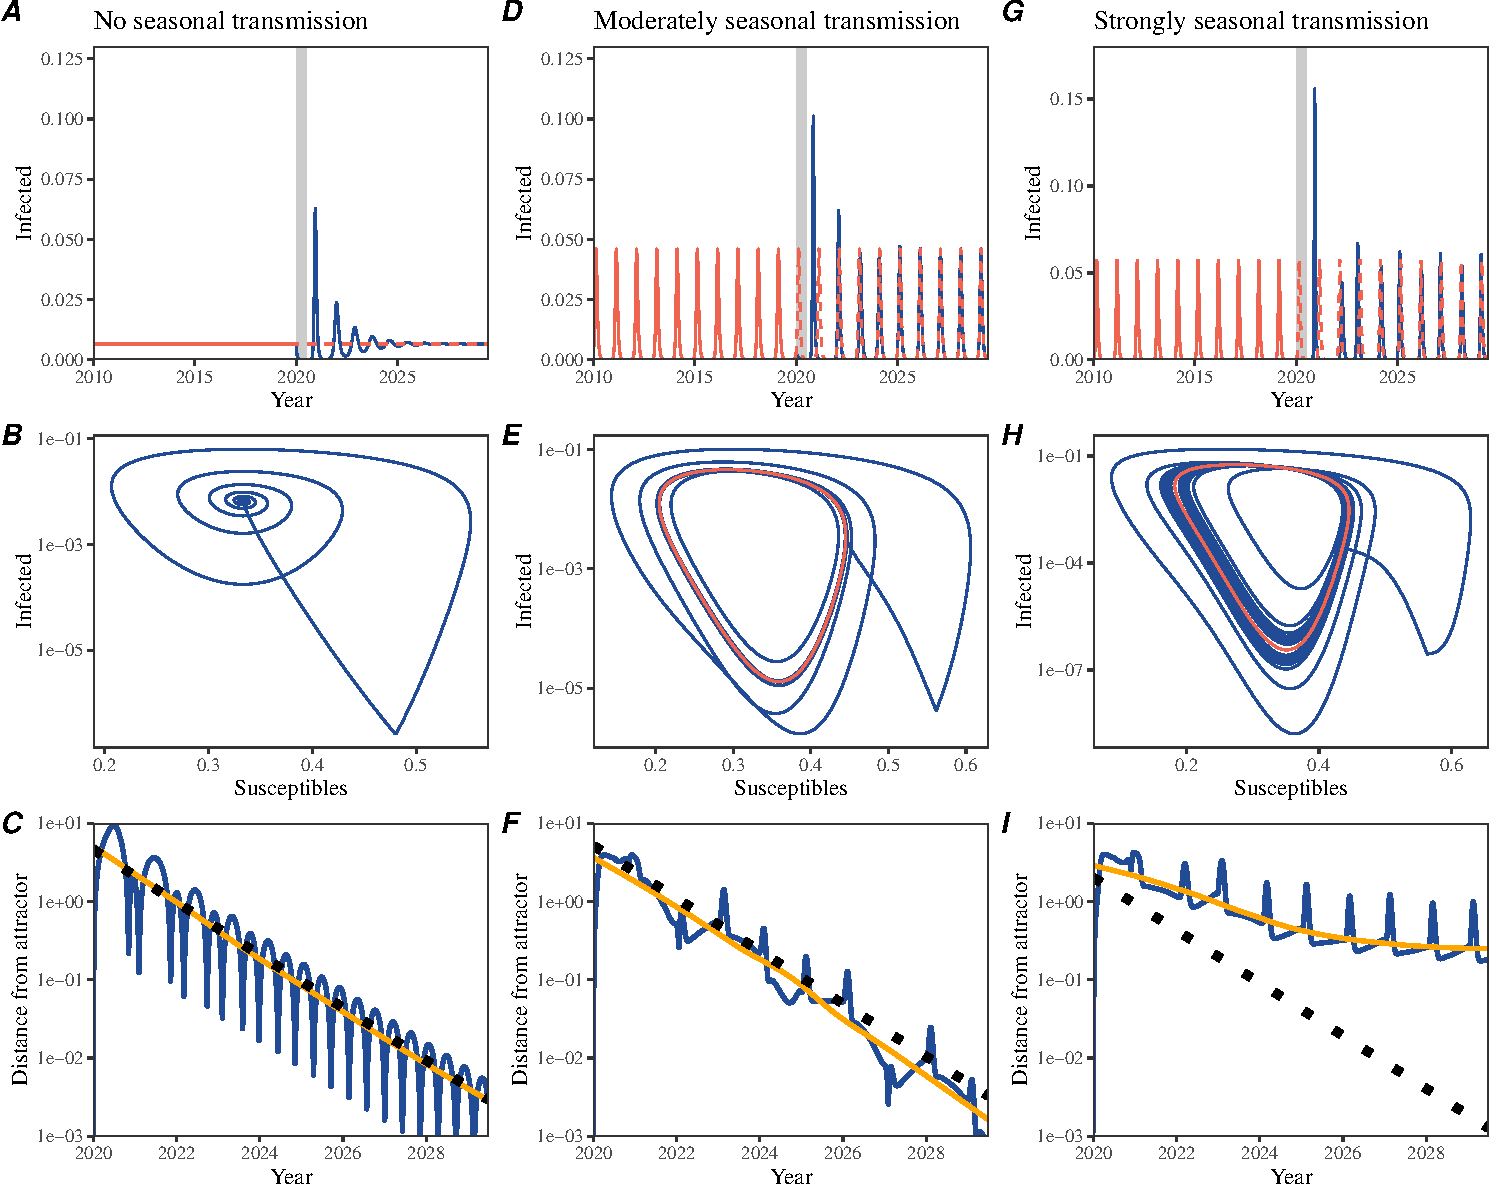
\includegraphics[width=\textwidth]{../figure2/figure2_simple_seas.pdf}
\caption{
\textbf{Impact of seasonal transmission on pathogen resilience.}
(A, D, G) Simulated epidemic trajectories using the SIRS model without seasonal forcing (A), with seasonal forcing of amplitude of 0.2 (D), and with seasonal forcing of amplitude of 0.2 (G).
Red and blue solid lines represent epidemic dynamics before and after interventions are introduced, respectively.
Red dashed lines represent counterfactual epidemic dynamics in the absence of interventions.
Gray regions indicate the duration of interventions.
(B, E, H) Phase plane representation of the corresponding model.
Red and blue solid lines represent epidemic trajectories on an SI phase plane before and after interventions are introduced, respectively.
(C, F, I) Changes in logged distance from attractor over time.
Blue lines represent the logged distance from attractor.
Orange lines represent the locally estimated scatterplot smoothing (LOESS) fits to the logged distance from attractor.
Dotted lines are superimposed as a comparison to have the same slope as the intrinsic resilience of the seasonally unforced system.
}
\end{figure}

\pagebreak

\begin{figure}[!th]
\includegraphics[width=\textwidth]{../figure2/figure2_multi_noseas.pdf}
\caption{
\textbf{Conceptual framework for measuring pathogen resilience following NPIs for a multi-strain system without seasonal forcing.}
(A, D, G) Simulated epidemic trajectories using a multi-strain system without seasonal forcing.
Red and blue solid lines represent epidemic dynamics before and after interventions are introduced, respectively.
Red dashed lines represent counterfactual epidemic dynamics in the absence of interventions.
Gray regions indicate the duration of interventions.
(B, E, H) Phase plane representation of the corresponding model.
Red and blue solid lines represent epidemic trajectories on an SI phase plane before and after interventions are introduced, respectively.
(C, F, I) Changes in logged distance from attractor over time.
Blue lines represent the logged distance from attractor.
Orange lines represent the locally estimated scatterplot smoothing (LOESS) fits to the logged distance from attractor.
Dotted lines are superimposed as a comparison to have the same slope as the intrinsic resilience of the seasonally unforced system.
}
\end{figure}

\pagebreak

\begin{figure}[!th]
\includegraphics[width=\textwidth]{../figure2/figure2_multi.pdf}
\caption{
\textbf{Conceptual framework for measuring pathogen resilience following NPIs for a multi-strain system with seasonal forcing.}
(A, D, G) Simulated epidemic trajectories using a multi-strain system with seasonal forcing (amplitude of 0.2).
Red and blue solid lines represent epidemic dynamics before and after interventions are introduced, respectively.
Red dashed lines represent counterfactual epidemic dynamics in the absence of interventions.
Gray regions indicate the duration of interventions.
(B, E, H) Phase plane representation of the corresponding model.
Red and blue solid lines represent epidemic trajectories on an SI phase plane before and after interventions are introduced, respectively.
(C, F, I) Changes in logged distance from attractor over time.
Blue lines represent the logged distance from attractor.
Orange lines represent the locally estimated scatterplot smoothing (LOESS) fits to the logged distance from attractor.
Dotted lines are superimposed as a comparison to have the same slope as the intrinsic resilience of the seasonally unforced system.
}
\end{figure}

\pagebreak

\begin{figure}[!th]
\includegraphics[width=\textwidth]{../figure2/figure2_multi_strong.pdf}
\caption{
\textbf{Conceptual framework for measuring pathogen resilience following NPIs for a multi-strain system with strong seasonal forcing.}
(A, D, G) Simulated epidemic trajectories using a multi-strain system with seasonal forcing (amplitude of 0.4).
Red and blue solid lines represent epidemic dynamics before and after interventions are introduced, respectively.
Red dashed lines represent counterfactual epidemic dynamics in the absence of interventions.
Gray regions indicate the duration of interventions.
(B, E, H) Phase plane representation of the corresponding model.
Red and blue solid lines represent epidemic trajectories on an SI phase plane before and after interventions are introduced, respectively.
(C, F, I) Changes in logged distance from attractor over time.
Blue lines represent the logged distance from attractor.
Orange lines represent the locally estimated scatterplot smoothing (LOESS) fits to the logged distance from attractor.
Dotted lines are superimposed as a comparison to have the same slope as the intrinsic resilience of the seasonally unforced system.
}
\end{figure}

\pagebreak

\begin{figure}[!th]
\includegraphics[width=\textwidth]{../figure_fit/figure_fit.pdf}
\caption{
\textbf{Mechanistic model fits to simulated data and inferred intrinsic resilience.}
(A, D, G, J) Simulated case time series from corresponding models (red) and SIRS model fits (black).
(B, E, H, K) Assumed changes in transmission due to COVID-19 interventions (red) and estimated changes from the SIRS model (black).
Solid lines and shaded regions represent fitted posterior median and 95\% credible intervals.
(C, F, I, L) True intrinsic resilience of the seasonally unforced system (vertical lines) and the posterior distribution of the inferred intrinsic resilience from the SIRS model (density plots).
}
\end{figure}


\pagebreak

\begin{figure}[!th]
\includegraphics[width=\textwidth]{../figure3/figure3_sens.pdf}
\caption{
\textbf{Sensitivity of the distance from attractor to choices about emedding lags and dimensions.}
Sensitivity analysis for the distance-from-attractor time series shown in Figure 3E in the main text by varying the embedding lag between 10--15 days and embedding dimensions between 2--6 dimensions.
}
\end{figure}

\pagebreak

\begin{figure}[!th]
\includegraphics[width=\textwidth]{../figure_analysis_random/figure_analysis_random.pdf}
\caption{
\textbf{Impact of fitting window selection on the estimation of empirical resilience.}
We simulate 500 epidemics using stochastic SIRS model with randomly drawn parameters and randomly generated intervention impacts.
For each simulation, we reconstruct the empirical attractor based on the approach outlined in Figure 3 and estimate the distance from attractor.
The naive approach fits a linear regression on a log scale, starting from the maximum distance until the end of the time series.
The window-based approach tries to select an appropriate window by smoothing the distance estimates and finding a time period when the smoothed time series crosses pre-determined threshold, relatively to the maximum distance;
then, a linear regression is fitted by using the raw distance within this time period.
}
\end{figure}

\pagebreak

\begin{figure}[!th]
\includegraphics[width=\textwidth]{../figure4/figure4_dist.pdf}
\caption{
\textbf{Estimated time series of distance from attractor for each pathogen across Canada, Hong Kong, Korea, and the US.}
Black lines represent the estimated distance from attractor.
Red lines and shaded regions represent the linear regression fits and corresponding 95\% confidence intervals.
Dashed lines represent the average of the pre-pandemic nearest neighbor distances.
}
\end{figure}

\pagebreak

\begin{figure}[!th]
\includegraphics[width=\textwidth]{../figure4/figure4_unzoom.pdf}
\caption{
\textbf{Predicted timing of when each pathogen will return to their pre-pandemic cycles (zoomed out).}
The dashed line in panel B indicates the end of 2024 (current observation time).
Error bars represent 95\% confidence intervals.
}
\end{figure}

\pagebreak

\begin{figure}[!th]
\includegraphics[width=\textwidth]{../figure4_th/figure4_dist_th.pdf}
\caption{
\textbf{Estimated time series of distance from attractor for each pathogen across Canada, Hong Kong, Korea, and the US using higher embedding dimensions.}
Black lines represent the estimated distance from attractor.
Red lines and shaded regions represent the linear regression fits and corresponding 95\% confidence intervals.
Dashed lines represent the average of the pre-pandemic nearest neighbor distances.
A lower threshold is used for determining embedding dimensions with the false nearest neighbors approach, thereby yielding a higher embedding dimension.
}
\end{figure}

\pagebreak

\begin{figure}[!th]
\begin{center}
\includegraphics[width=0.8\textwidth]{../figure4_th/figure4_th.pdf}
\caption{
\textbf{Summary of resilience estimates using higher embedding dimensions.}
(A) Estimated pathogen resilience.
The gray horizontal line represents the intrinsic resilience of pre-vaccination measles dynamics.
(B) Predicted timing of when each pathogen will return to their pre-pandemic cycles.
The dashed line in panel B indicates the end of 2024 (current observation time).
Error bars represent 95\% confidence intervals.
A lower threshold is used for determining embedding dimensions with the false nearest neighbors approach, thereby yielding a higher embedding dimension.
}
\end{center}
\end{figure}

\pagebreak

\begin{figure}[!th]
\begin{center}
\includegraphics[width=0.8\textwidth]{../figure4_th/figure4_comparison.pdf}
\caption{
\textbf{Comparison of resilience estimates.}
Each point represents a resilience estimate for a specific pathogen at a specific country.
The x values represent the original resilience estimates presented in Figure 4.
The y values represent the original resilience estimates presented in Supplementary Figure S11.
}
\end{center}
\end{figure}

\pagebreak


\bibliography{return-time.bib}

\end{document}
